\chapter{LMS7002M}

\begin{figure}[h!]
\centering
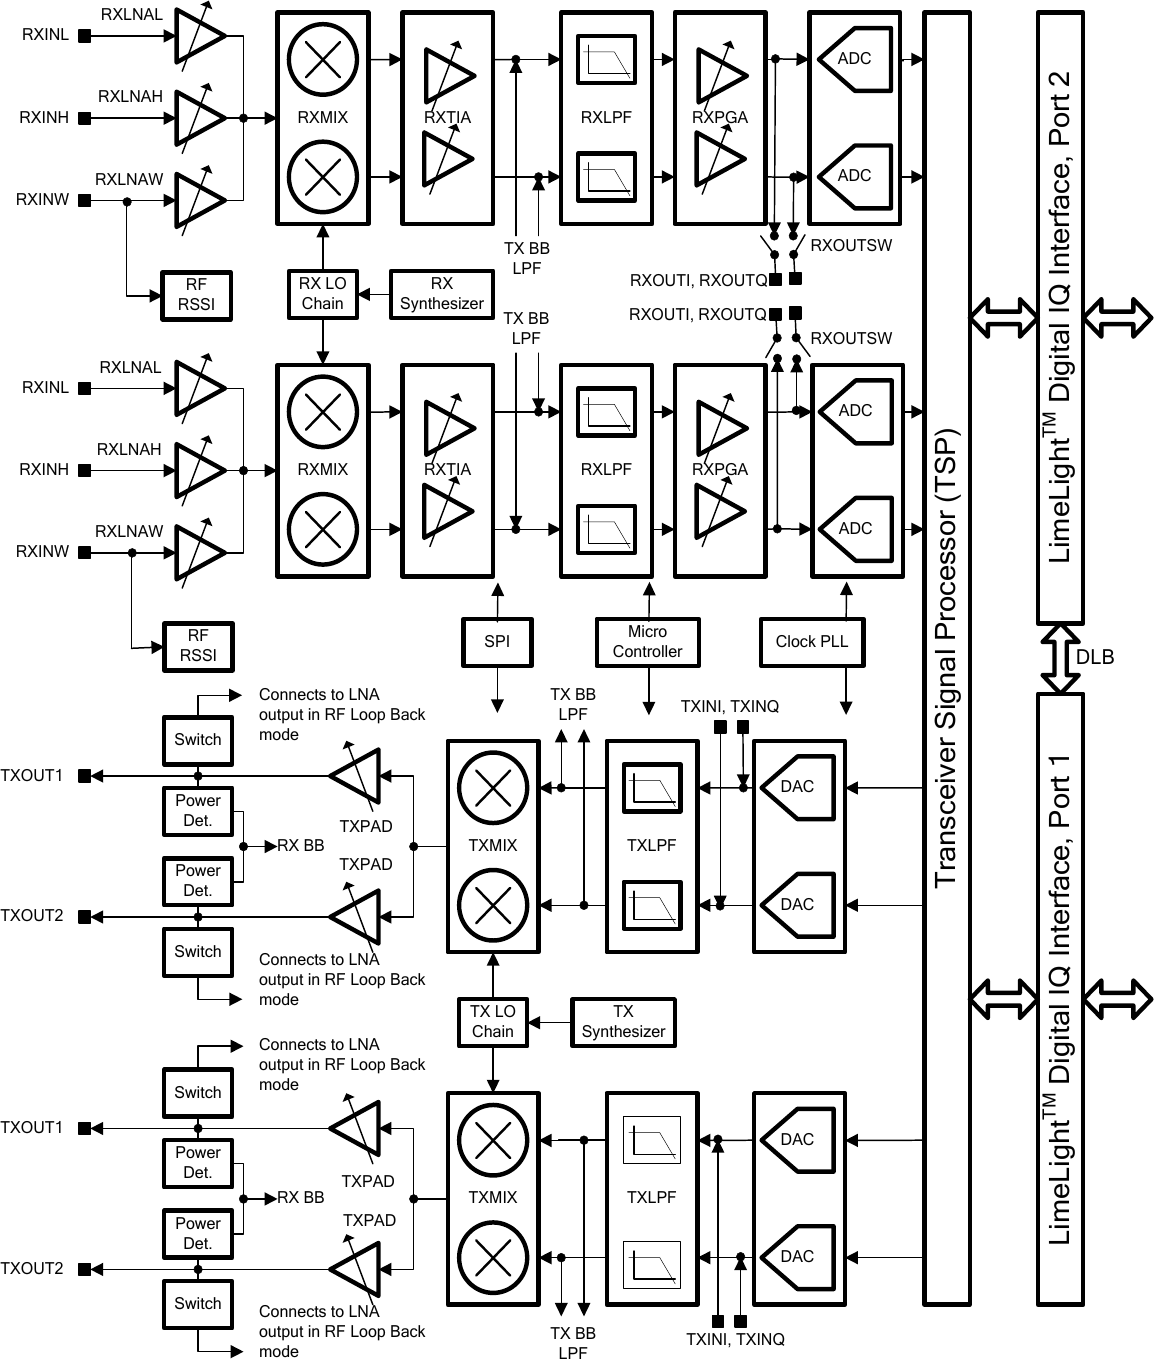
\includegraphics[width=0.9\textwidth]{Figure/Lms7002m-block-diagram.png}
\caption{Block Diagram of LMS7002M.}
\label{lms7002m}
\end{figure}

LMS7002M offers full duplex communication link on both the TX and RX chains.
Each of the RX chains has three separate \ac{RF} ports tuned for narrow band low frequency, narrow band high frequency and wide band operations.
Similarly, the TX Chains are connected two separate \ac{RF} ports tuned for high frequency and low frequency operations.
This separation is done for better impedance matching at the boundary of the antennas.\\

Figure \ref{lms7002m} shows the functional block diagram for a LMS7002M \ac{FPRF}.
Since, both the RX and TX paths are identical, the report concentrates on only one RX path.
The output from the \ac{RF} RX ports are fed into the \ac{LNA} inorder to minimize injecting too much noise at the beginning of the chain.
The receiver follows the architecture shown in Figure \ref{rf_receiver}, with a RX mixer, followed by filter and a \ac{PGA} combined in a Zero-IF architecture.
The RX \ac{PGA} outputs the analog baseband signal.\\

LMS7002M uses a fractional N-\ac{PLL} architecture for the local oscillator frequency synthesis.
\ac{PLL} is used extensively in \ac{RF} circuits for making sure the generated local oscillator signal and the reference signal have the same phase and frequency.
PLLs are essentially negative feedback systems, so when the input signal differs a lot from the output signal, the control logic tries to lower the error (\textit{input-output)}.\\

Integer N- \ac{PLL} architectures are used to generate high frequency signals from low frequency reference clocks, by using a frequency divider in the negative loopback path.
The frequency divider is basically a counter, that outputs every "N" (division factor of the loop) clock cycles of the output signal.
But since the output signal frequency will be multiples of the reference clock, the output signal resolution is determined by the  reference clock.\\

So to have a high frequency as well as a high resolution, the divider counter should be very large in size.
To counter the problem, fractional N-{PLL} architectures were designed where the output signal frequency can also be a fractional multiple of the input signal frequency.
This helps in increasing the frequency resolution without the need for a large divisor counter.
The input and output frequency relationship for a fractional  N-\ac{PLL} can be summarized by: $f_{out}=f_{ref}(N+k/M)$, where N is the integer divider factor, k is the fractional divider factor and $1/M$ gives the output frequency resolution.
Both the integer and fractional divider factor are determined by the size of the counters used.
In case of LimeSDR, the reference signal fed to the PLL varies from to 10 to 52 MHz.
The output signal can vary from 30 to 3800 MHz, with a frequency resolution of 24.8 Hz.\\

Once the \ac{RF} demodulation is completed by the analog processing chain, the analog signal is sent to the data converters and converted to digital data samples.
The sampling rate for the data conversion is determined by the required \ac{RF} channel bandwidth.
The digital samples are sent to the \ac{TSP} for further processing.\\

The \ac{TSP} uses advanced signal processing algorithms like IQ DC offset correction, IQ phase correction for correcting the received samples.
An interpolation and decimation filter is added to the \ac{TSP} for the TX and RX chains respectively.
These filters are implemented with a chain of five fixed co-efficient half band \ac{FIR} filters, which allows interpolation and decimation factors of 1,2,4,8,16.
Interpolation and Decimation allows the baseband to run at a lower data rate while still running the data converters at higher sampling rates, enabling the quantization noise to be spread over larger frequency range.
Automatic Gain Control is also implemented by the the \ac{TSP}.\\